%%%%%%%%%%%%%%%%%%%%%%%%%%%%%%%%%%%%%%%%%%%%%%%%%%%%%%%%%%%%%%%%%%%%%%%
% Universidade Federal de Santa Catarina             
% Biblioteca Universit�ria                     
%----------------------------------------------------------------------
% Exemplo de utiliza��o da documentclass ufscThesis
%----------------------------------------------------------------------                                                           
% (c)2013 Roberto Simoni (roberto.emc@gmail.com)
%         Carlos R Rocha (cticarlo@gmail.com)
%         Rafael M Casali (rafaelmcasali@yahoo.com.br)
%%%%%%%%%%%%%%%%%%%%%%%%%%%%%%%%%%%%%%%%%%%%%%%%%%%%%%%%%%%%%%%%%%%%%%%
\documentclass{ufscThesis} % Definicao do documentclass ufscThesis	

%----------------------------------------------------------------------
% Pacotes usados especificamente neste documento
\usepackage{graphicx} % Possibilita o uso de figuras e gr�ficos
\usepackage{color}    % Possibilita o uso de cores no documento
\usepackage{listings}
%----------------------------------------------------------------------
% Comandos criados pelo usu�rio
\newcommand{\afazer}[1]{{\color{red}{#1}}} % Para destacar uma parte a ser trabalhada
\newcommand{\ABNTbibliographyname}{REFER�NCIAS}

%----------------------------------------------------------------------

% Identificadores do trabalho
% Usados para preencher os elementos pré-textuais

\instituicao[a]{Universidade Federal de Santa Catarina} % Opcional
\departamento[o]{INE}
\curso[o]{curso de Ciências da Computação}
\documento[o]{TCC} % [o] para dissertação [a] para tese
\titulo{Proposta de uma plataforma de sistema multiagente para suportar ações visando otimização energética em ambientes de computação em nuvem}
\autor{Lucas Berri Cristofolini}
\grau{Bacharel}
\local{Florianópolis} % Opcional (Florianópolis é o padrão)
\data{23}{agosto}{2015}
\orientador[Orientador\\Universidade Federal de Santa Catarina]{Prof. Dr. Ricardo Azambuja Silveira}
\coorientador[Coorientador\\Universidade Federal de Santa Catarina]{Rafael Weingärtner}
\coordenador[Coordenador\\Universidade Federal de Santa Catarina]{Prof. Dr. Renato Cislaghi}

\numerodemembrosnabanca{4} % Isso decide se haverá uma folha adicional
\orientadornabanca{nao} % Se faz parte da banca definir como sim
\coorientadornabanca{sim} % Se faz parte da banca definir como sim
\bancaMembroA{Primeiro membro\\Universidade ...} %Nome do presidente da banca
\bancaMembroB{Segundo membro\\Universidade ...}      % Nome do membro da Banca
\bancaMembroC{Terceiro membro\\Universidade ...}     % Nome do membro da Banca
%\bancaMembroD{Quarto membro\\Universidade ...}       % Nome do membro da Banca
%\bancaMembroE{Quinto membro\\Universidade ...}       % Nome do membro da Banca
%\bancaMembroF{Sexto membro\\Universidade ...}        % Nome do membro da Banca
%\bancaMembroG{Sétimo membro\\Universidade ...}       % Nome do membro da Banca

\dedicatoria{Este trabalho é dedicado aos meus colegas de classe e aos meus queridos pais.}

\agradecimento{Inserir os agradecimentos aos colaboradores à execução do trabalho.}

\epigrafe{Texto da Epígrafe. Citação relativa ao tema do trabalho. É opcional. A epígrafe pode também aparecer na abertura de cada seção ou capítulo.}
{(Autor da epígrafe, ano)}

\textoResumo {Dada a complexidade, heterogeneidade e dinamismo crescentes presentes nos ambientes de computa��o em nuvem, otimizar a utiliza��o de recursos nestes ambientes torna-se uma tarefa desafiadora. Motivado pela semelhan�a entre entre os paradigmas de computa��o em nuvem e sistemas multiagentes, este trabalho se prop�em a adaptar uma ferramenta de orquestra��o existente, de modo a utilizar uma plataforma de sistemas multiagentes para possibilitar que agentes inteligentes realizem a an�lise, o planejamento e a ger�ncia em ambientes de computa��o em nuvem de forma independente e aut�noma.}
\palavrasChave {Computa��o em Nuvem. Int�ligencia Artificial.  Sistemas multiagentes. Orquestra��o de computa��o em nuvem}
 
\textAbstract {Given the complexity, heterogeneity and growing dynamism presented on cloud computing environments, the optimization on resource usage in aforementioned environments turns into a challenging task. Driven by the similarities between cloud computing paradigm and multiagent systems, this work proposes adaptations within an existing orchestration tool, so it can make use of a multiagent systems's platform, enabling intelligent agents to handle the analysis, planning and management of cloud computing environments in an independent and autonomous fashion.}
\keywords {Cloud Computing. Artificial Intelligence. Multiagent Systems}


%----------------------------------------------------------------------
% In�cio do documento                                
\begin{document}
%--------------------------------------------------------
% Elementos pr�-textuais
%\capa  
% BOTAR DEPOIS \folhaderosto % Se nao quiser imprimir a ficha, � s� n�o usar o par�metro
%\folhaaprovacao
%\paginadedicatoria
%\paginaagradecimento
%\paginaepigrafe
% BOTAR DEPOIS \paginaresumo
% BOTAR DEPOIS \paginaabstract
%\pretextuais % Substitui todos os elementos pre-textuais acima
%\listadefiguras % as listas dependem da necessidade do usu�rio
%\listadetabelas 
% BOTAR DEPOIS \listadeabreviaturas
% BOTAR DEPOIS \listadesimbolos
% BOTAR DEPOIS \sumario 
%--------------------------------------------------------
% Elementos textuais

\chapter{Introdu��o}
% NOVA

Computa��o em nuvem (CN)\abreviatura{CN}{Computa��o em nuvem} � um paradigma tecnol�gico, que vem chamando a aten��o dos provedores de servi�os, por propor uma mudan�a na forma de disponibilizar seus produtos. A grande aceita��o aos servi�os de CN vista recentemente se deve, entre outros motivos, � n�o necessidade de um grande investimento inicial, sendo que os clientes que buscam esse servi�o pagam apenas pelo que utilizam \cite{payg}. A ado��o do paradigma � uma tend�ncia observada em empresas de pequeno � grande porte, sendo as principais raz�es, melhorar a disponibilidade dos seus servi�os al�m de obter uma melhora na infra-estrutura interna \cite{instance1290}.\par

 Os benef�cios da CN est�o altamente ligados com a qualidade de servi�o (QoS) \abreviatura{QoS}{Qualidade de Servi�o}percebida pelos usu�rios. A necessidade de entregar QoS aos consumidores faz com que recursos sejam mantidos ociosos a espera de cargas estoc�sticas, consumindo mais energia e influenciando diretamente nos custos de manuten��o de um ambiente na nuvem \cite{forecasting}.\par

 Uma alternativa para reduzir este consumo desnecess�rio em um ambiente de CN consiste em aglomerar as m�quinas virtuais ativas no menor n�mero de servidores f�sicos, possibilitando desligar os recursos ociosos e lig�-los quando a demanda por recursos tornar-se necess�ria \cite{consolidation}. Entretanto, dada a falta de suporte a medidas de gerenciamento energ�tico nas ferramentas de orquestra��o de ambientes de CN dispon�veis atualmente, \citeonline{gabriel} propos a ado��o de um \emph{framework} para a consolida��o de recursos em ambientes de CN visando uma melhor efici�ncia energ�tica do ambiente  orquestrado. A proposta consiste na implementa��o de um gerente de consolida��o baseado em heur�sticas pr�-definidas para agrupar m�quinas virtuais no menor n�mero de servidores f�sicos poss�veis para poder desativar servidores sem carga.\par 

Problemas como este, onde n�o se conhece uma f�rmula para obter a melhor solu��o e onde a informa��o est� distribu�da pelo ambiente podem ser tratados atrav�s de uma abordadem de sistemas multiagentes (SMA)\abreviatura{SMA}{Sistemas Multiagente}. Dessa forma � poss�vel trabalhar de forma h�brida em cima do problema \cite{a-ricardo-intro}, trazendo o conhecimento de um especialista para os agentes do ambiente, que por sua vez atuar�o para alcan�ar seus objetivos. Adicionado a isto, a natureza heterog�nea, din�mica e cont�nua de SMA, semelhante a de CN, faz com que pare�a natural e condizente uma converg�ncia entre as t�cnologias. 


\section{Motiva��o e Justificativa}
Ambientes de computa��o em nuvem mant�m recursos ociosos ativos visando manter a disponibilidade e a qualidade do servi�o em momentos de aumento s�bito de utiliza��o de recursos \cite{gabriel}. Isso faz com que o consumo energ�tico destes ambientes seja elevado, causando um impacto consider�vel nas despesas envolvidas em manuten��o bem como no meio ambiente, considerando que apenas 21\% de toda energia produzida mundialmente procede de fontes renov�veis \cite{ieo2013}. \par

A energia usada por um servidor ligado n�o � linearmente proporcional a carga com que ele est� trabalhando, como observado em \citeonline{awada2014energy}. Pontos levantados na pesquisa realizada por Awada, Li e Shen servem de motiva��o para o estudo de t�cnicas para ger�ncia de ambientes na nuvem, entre eles, alguns merecem destaque \cite{gabriel}:

\begin{itemize}  
	\item Os servidores, mesmo com 20\% de carga, tendem a consumir 80\% da energia necess�ria quando exigidos ao m�ximo;
	\item Servidores, avaliados em ambientes reais, no geral s�o expostos a cargas de uso entre 10\% e 50\%;
	\item O custo para refrigerac�o destes ambientes, reflete em 30\% do custo energ�tico total do centro de processamento.
\end{itemize}

Esses dados mostram que � necess�rio uma melhor ger�ncia dos recursos dispon�veis. Um centro de processamento de dados que possui servidores sub-utilizadas, torna-se ineficiente, tanto energeticamente quanto pelo poder computacional ocioso. At� ent�o, nenhuma das ferramentas de orquestra��o de CN mais conhecidas e dispon�veis no mercado avaliadas por \citeonline{gabriel} possuem funcionalidades voltadas � ger�ncia do consumo energ�tico nos ambientes orquestrados. Tal cen�rio faz com que empresas de pequeno e m�dio porte, representando mais do que 90\% do consumo energ�tico total utilizado para alimenta��o e refrigera��o de \emph{datacenters} americanos, tenham dificuldades para gerenciar o consumo energ�tico dos seus centros de processamento de dados \cite{whitney2014data}.\par

Seguindo os passos de agentes informais de consolida��o j� propostos e testados por Uchechukwu, Li e Shen, que mostram resultados de diminui��o de m�quinas ativas de 81\% para 44\% \cite{uchechukwu2012improving}, pode-se pensar em uma implementa��o formal, com par�metros vari�veis de QoS, usando t�cnicas de sistemas multiagentes.\par

Por mais que o uso de agentes na nuvem tenha sido, at� agora, limitado a SMAs que usam recursos computacionais da nuvem e nuvens que utilizam SMA para prover servi�os inteligentes \cite{mascloud}. \citeonline{wooldridge2009introduction} pontua que o uso de uma abordagem multiagentes � recomendada quando o problema possui um ambiente aberto, din�mico e complexo, ou tamb�m quando existem dados, controle e expertise distribuidos no ambiente. \par

Tendo em vista a adequa��o de um sistema multiagente a um meio heterog�neo como a orquestra��o de um ambiente de CN, surgiu o interesse em expandir o \emph{framework} proposto por \citeonline{gabriel} com a ado��o de uma plataforma multiagente que viria a substituir o agente implementado. Assim, flexibiliza-se a adapta��o dos agentes para a execu��o de diferentes a��es nas diferentes partes que comp�em a ferramenta de orquestra��o, visando uma maior especificidade e paraleliza��o das tarefas a serem adotadas. \par

A ado��o de uma plataforma multiagente permitir� a implementa��o de diferentes agentes que atuar�o em partes heterog�neas distintas que comp�em um ambiente de CN. Al�m de serem adaptados a �reas espec�ficas do ambiente, esses agentes ter�o a capacidade de se comunicar, permitindo que sejam voltados para uma parte do ambiente onde possam reagir adequadamente a ocorr�ncias de eventos. Diferentes agentes poder�o ser inicializados e removidos de acordo com a demanda do ambiente no qual forem implementados. \par


\section{Objetivos}
\subsection{Objetivo Geral}


\subsection{Objetivos Específicos}


\chapter{Fundamenta��o}

Neste cap�tulo ser�o introduzidos conceitos abordados no decorrer do trabalho.

\subsection{Virtualiza��o}
Segundo \citeonline{tholeti2011hypervisors}, virtualiza��o � definida como a cria��o de substitutos para os verdadeiros recursos f�sicos podendo ser criados a partir de divis�es l�gicas. Estes possuem a mesma fun��o e interfaces dos recursos f�sicos, mas diferem em tamanho, performance e custo. Os usu�rios destes recursos virtuais t�picamente n�o percebem a substitui��o, uma vez que sistemas virtuais devem obter performance semelhante a sua contraparte f�sica, em rela��o �s aplica��es dentro do servidor. Usando virtualiza��o � poss�vel fazer com que um recurso f�sico seja visto como m�ltiplos recursos virtuais. A Figura \ref{fig:virtualizacao} demonstra a cria��o de m�ltiplos sistemas virtuais independentes, que usam recursos virtuais, sobre um �nico sistema f�sico.

\begin{figure}[!htb]
 	\centering
 	\caption{Apresenta��o de um ambiente virtualizado, obtido de \cite{tholeti2011hypervisors}.}\label{fig:virtualizacao}
 	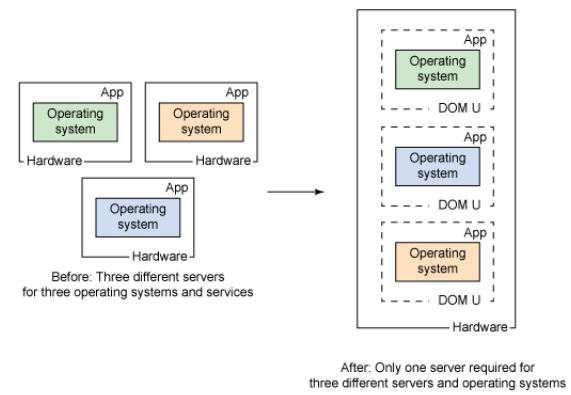
\includegraphics[width=1\textwidth]{figuras/virtualizacao.png}
\end{figure}


Os virtualizadores s�o componentes de software ou firmware capazes de virtualizar recursos f�sicos. Existem tr�s tipos de virtualiza��o diferentes, suas defini��es segundo \citeonline{tholeti2011hypervisors} s�o:

\begin{itemize}
	\item Tipo 1: a virtualiza��o de tipo 1 � caracterizada quando o virtualizador � executado diretamente sobre o hardware do sistema. Este m�todo � mais eficiente, tendo o melhor desempenho entre os m�todos de virtualiza��o;

	\item Tipo 2: a virtualiza��o de tipo 2 � caracterizada quando o virtualizador � executado sobre um sistema operacional hospedeiro que providencia servi�os de virtualiza��o, tais como suporte � entrada/sa�da de dados e gerenciamento de mem�ria;

	\item Virtualiza��o por uso de containers: este modo de virtualiza��o � caracterizado pela abstin�ncia do virtualizador. A virtualiza��o ocorre a n�vel de sistema operacional\abreviatura{SO}{Sistema Operacional} (SO), o qual permite a virtualiza��o de inst�ncias suas. Este modo de virtualiza��o resulta num uso mais eficiente de mem�ria, sendo esta sua vantagem diante dos outros m�todos de virtualiza��o. Todavia, como todas inst�ncias virtuais s�o imagens do SO ra�z, todas as inst�ncias ser�o da mesma vers�o que o SO ra�z.

\end{itemize}

A virtualiza��o � um processo utilizado nos ambientes na nuvem para dividir l�gicamente os recursos f�sicos de um servidor, normalmente sendo usados virtualizadores como componente respons�vel pela cria��o, remo��o e gerenciamento das \textit{virtual machines} \abreviatura{VM}{\textit{Virtual Machine}}(VMs), em portugu�s, m�quinas virtuais. O uso de virtualizadores facilita o provisionamento de diferentes sistemas operacionais sem que eles estejam instalados diretamente nos servidores f�sicos. Outra vantagem da virtualiza��o est� na facilita��o do processo de migra��o de VMs em tempo de execu��o para outros servidores fisicos, facilitando o processo de manuten��o.


\bibliographystyle{ufscThesis/ufsc-alf}
\bibliography{bibliografia}

\end{document}